% --- Verzeichnisse ------------------------------------------------------
\chapter{Abbildungen}
\newpage

\begin{figure}[htp!]
        \centering
                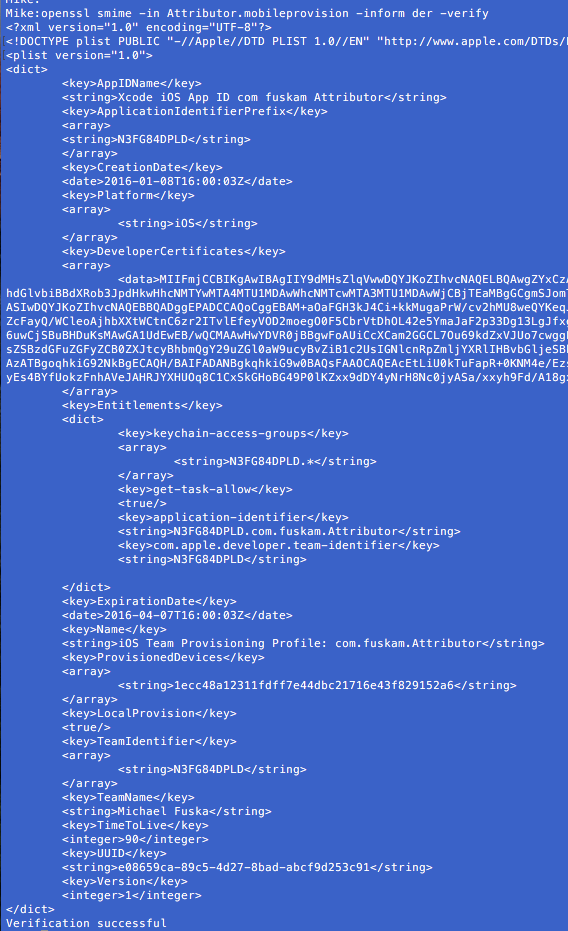
\includegraphics[scale=0.6]{SGML-Format}
        \caption{Provisioning Profile \protect\footnotemark}
        \label{fig:ProvisioningProfile}
\end{figure}
\footnotetext{Eigenwerk}
\newpage

\begin{figure}[htbp!]
        \centering
                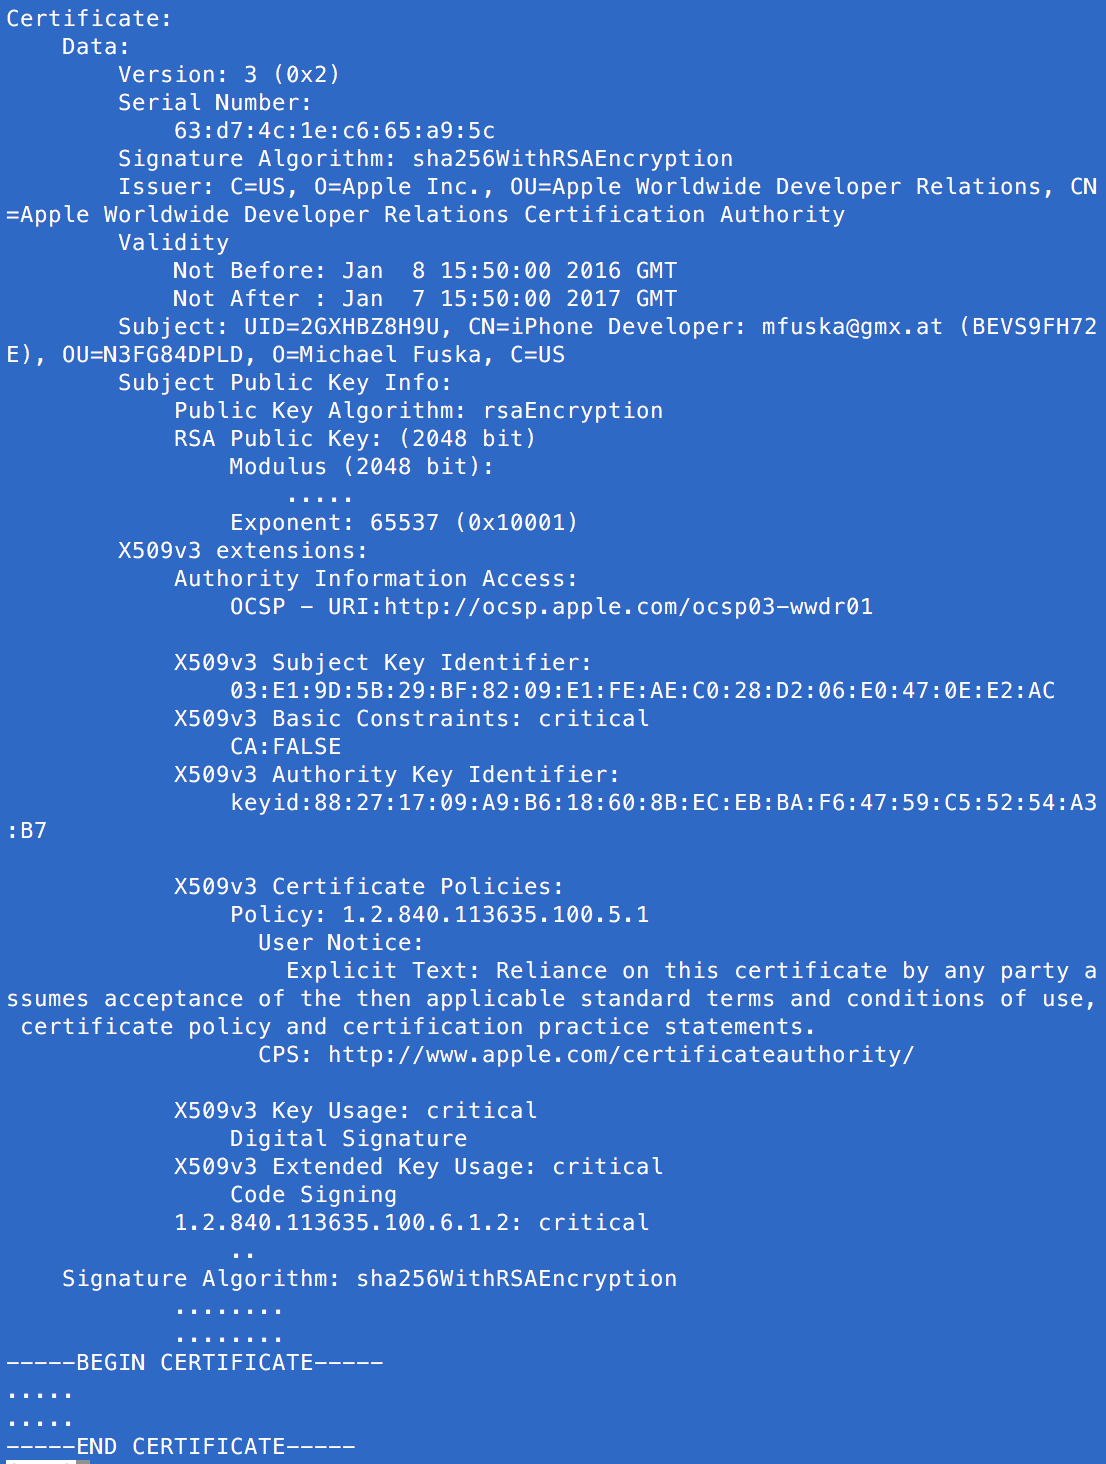
\includegraphics[scale=0.7]{Cert-output}
        \caption{Developer Certificates \protect\footnotemark}
        \label{fig:DeveloperCertificates}
\end{figure}
\footnotetext{Eigenwerk}
\newpage

\begin{figure}[htbp!]
    \centering 
		        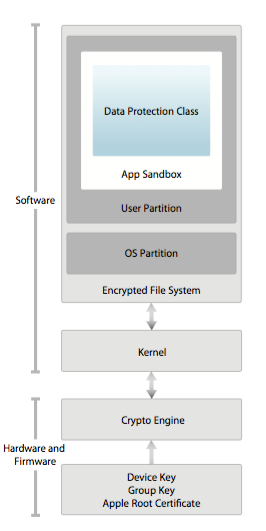
\includegraphics[scale=0.3]{Bilder/SecArchitektur-iOS7.png}
	\caption {iOS Security Architektur iPhone 5c (Quelle \cite{Apple[9]} S.3) } 
    \label{fig:iOSSecurityArchitekturiOS7}
\end{figure}

\begin{figure}[htbp!]
        \centering
                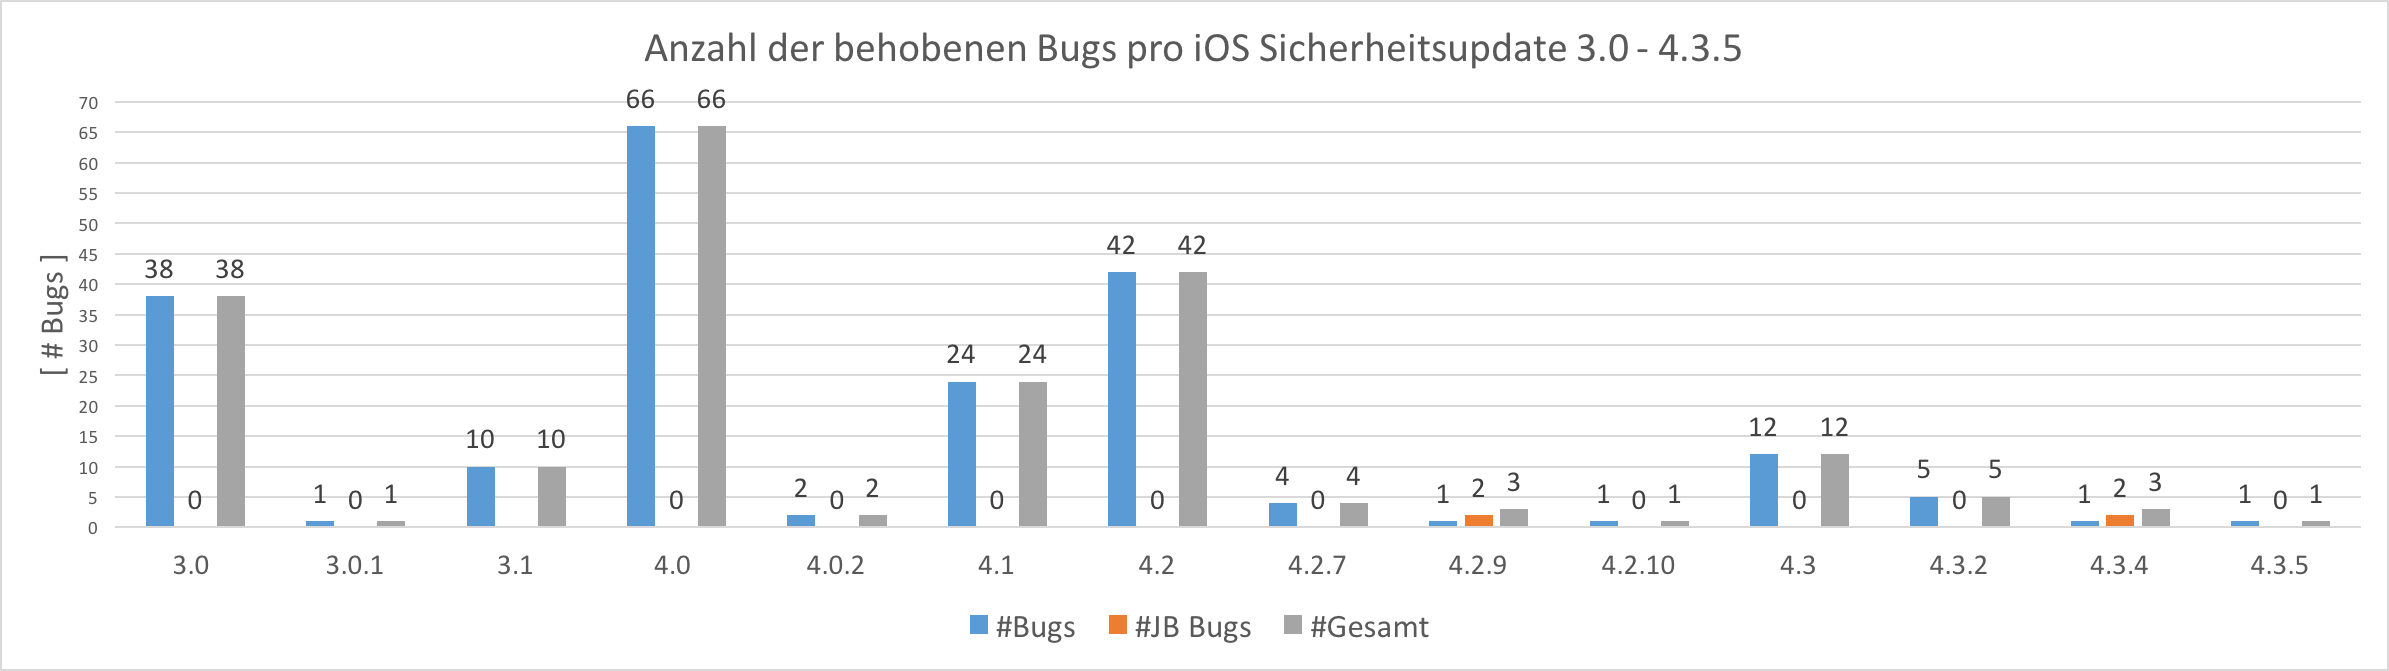
\includegraphics[scale=0.4]{Bilder/iOSSicherheitsupdate3.png}
        \caption{Anzahl der behobenen Bugs pro iOS-Sicherheitsupdates 3.x - 4.x \newline (vgl. \cite{Apple[7]}) \protect\footnotemark}
        \label{fig:AnalyseiOSSicherheitsupdate3}
\end{figure}
\footnotetext{Eigenwerk}

\begin{figure}[htbp!]
        \centering
                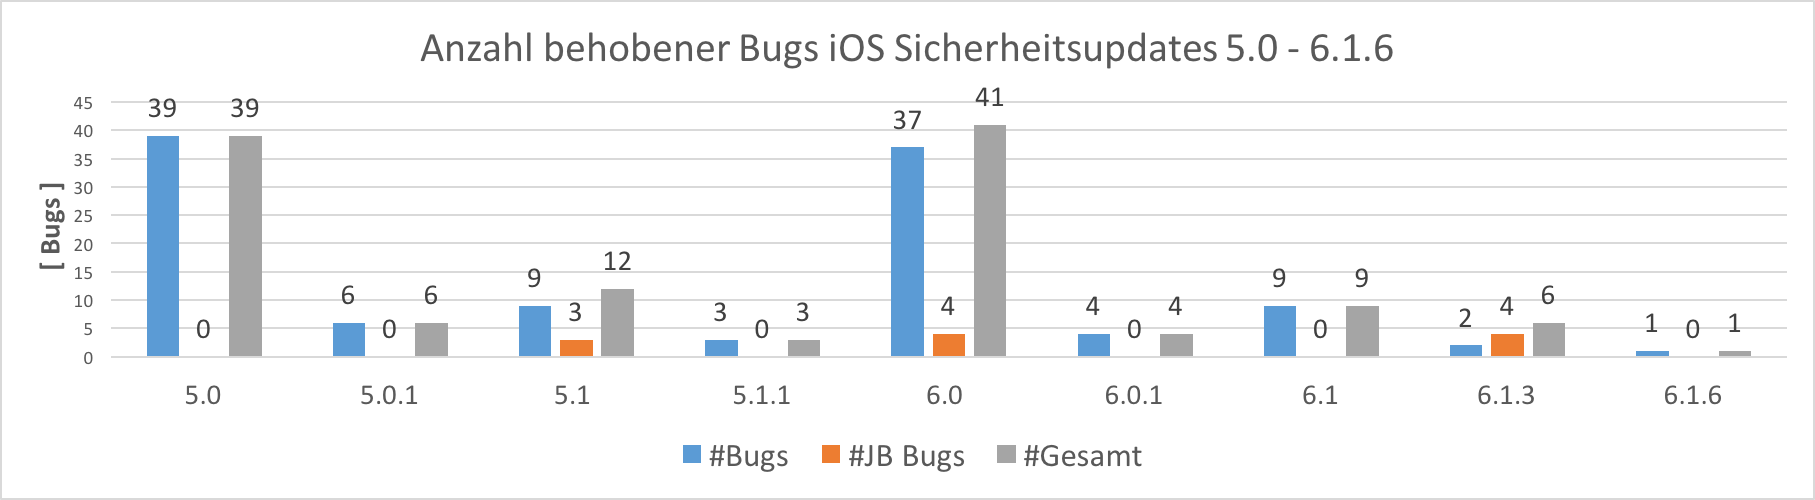
\includegraphics[scale=0.5]{Bilder/iOSSicherheitsupdate5.png}
        \caption{Anzahl der behobenen Bugs pro iOS-Sicherheitsupdates 5.x - 6.x \newline (vgl. \cite{Apple[7]}) \protect\footnotemark}
        \label{fig:AnalyseiOSSicherheitsupdate5}
\end{figure}
\footnotetext{Eigenwerk}

\newpage
\begin{figure}[htbp!]
        \centering
                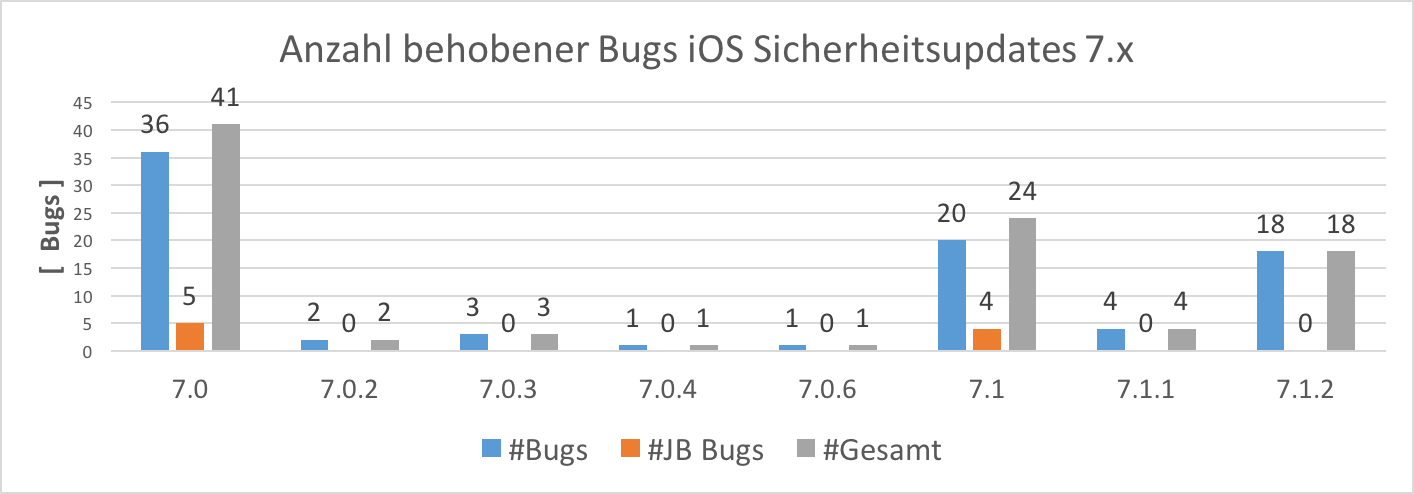
\includegraphics[scale=0.7]{Bilder/iOSSicherheitsupdate7.png}
        \caption{Anzahl der behobenen Bugs pro iOS-Sicherheitsupdates 7.x \newline (vgl. \cite{Apple[7]}) \protect\footnotemark}
        \label{fig:AnalyseiOSSicherheitsupdate7}
\end{figure}
\footnotetext{Eigenwerk}
\begin{figure}[htbp!]
        \centering
                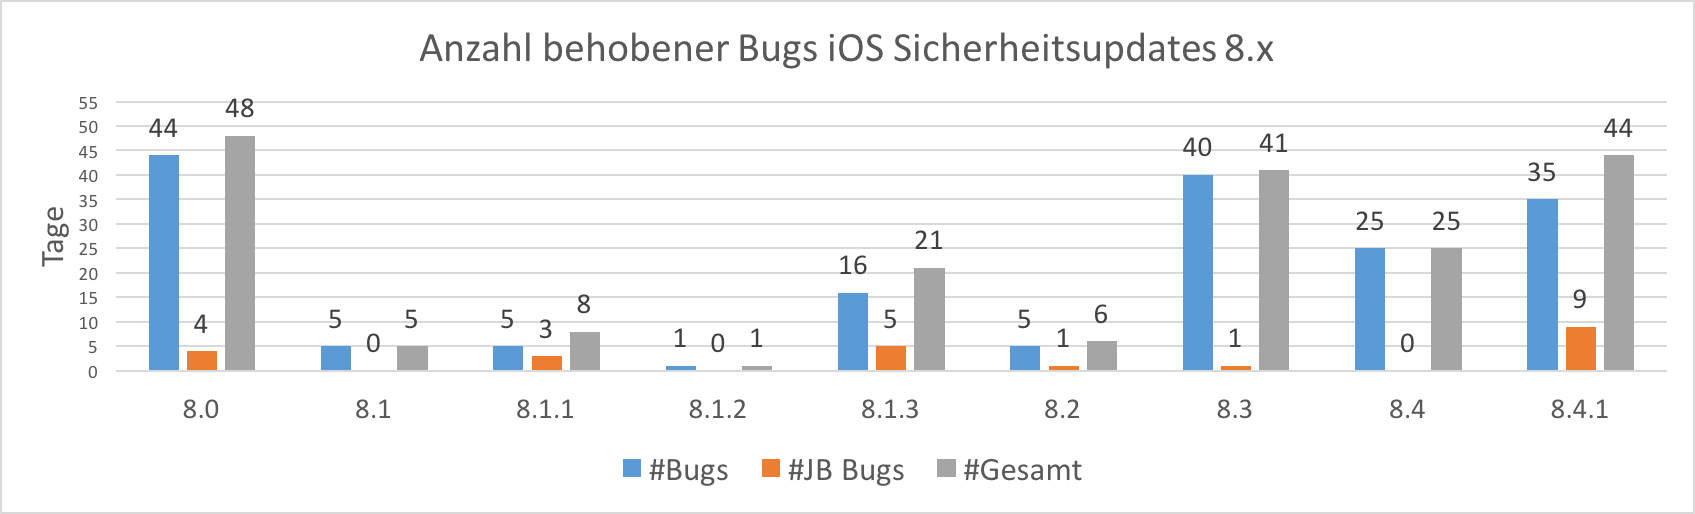
\includegraphics[scale=0.54]{Bilder/iOSSicherheitsupdate8.png}
        \caption{Anzahl der behobenen Bugs pro iOS-Sicherheitsupdates 8.x \newline (vgl. \cite{Apple[7]}) \protect\footnotemark}
        \label{fig:AnalyseiOSSicherheitsupdate8}
\end{figure}
\footnotetext{Eigenwerk}

\begin{figure}[ht!]
        \centering
                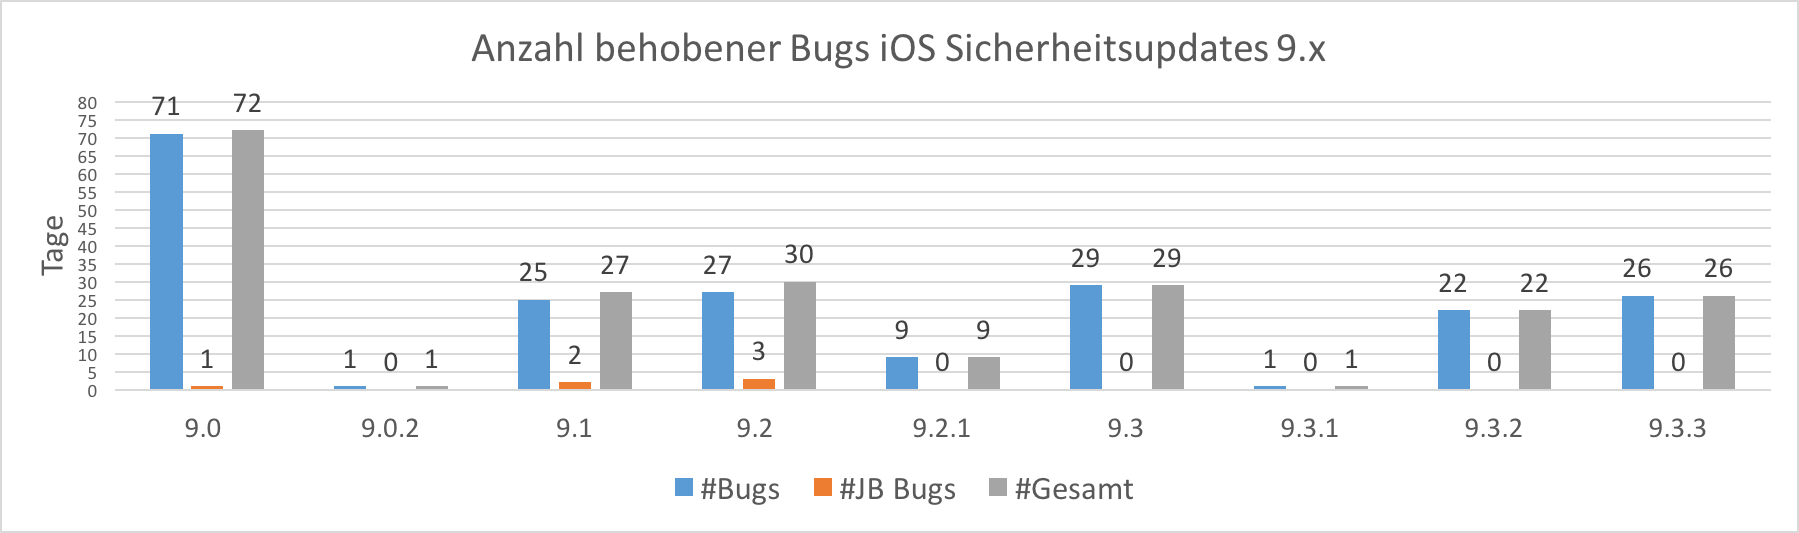
\includegraphics[scale=0.55]{Bilder/iOSSicherheitsupdate9.png}
        \caption{Anzahl der behobenen Bugs pro iOS-Sicherheitsupdates iOS 9.x \newline (vgl. \cite{Apple[7]}) \protect\footnotemark}
        \label{fig:AnalyseiOSSicherheitsupdate9}
\end{figure}
\footnotetext{Eigenwerk}
\newpage

\chapter{Tabellen}
\newpage

\begin{table}[htp!]
    \begin{center}
        \begin{tabular}{| p{8mm} | p{18mm} | p{18mm} | p{15mm} | p{15mm} | p{15mm} | p{15mm} | p{15mm} | p{15mm} |} \hline
\textbf{initial OS} & \textbf{Samsung S5L8900} & \textbf{Samsung S5L8920} & \textbf{Apple A4}	& \textbf{Apple A5}	& \textbf{Apple A6} & \textbf{Apple A7} & \textbf{Apple A8} & \textbf{Apple A9} \\ \hline
1.0 & iPhone & - & - &  - &  - & - &  - & - \\ \hline		
2.0 & iPhone 3G & - & - &  - &  - & - &  - & - \\ \hline				
3.0 & - & iPhone 3GS & - &  - &  - & - &  - & -	\\ \hline			
4.0 & - &  - & iPhone 4	 &  - &  - & - &  - & -	\\ \hline		
5.0 &  - & - &  - &	iPhone 4s &  - & - &  - & - \\ \hline		
6.0 &  - &  - & - &  - & iPhone 5 & - &  - & -	\\ \hline	
7.0 &  - &  - & - &  - & iPhone 5c	& - &  - & - \\ \hline	
7.0 & - &  - &  - & - &  - & iPhone 5s &  - & - \\ \hline
8.0 & - & - &  - &  - & - &  - & iPhone 6 & - \\ \hline
8.0 & - & - &  - &  - & - &  - & iPhone 6 Plus & -\\ \hline
9.0 & - & - &  - &  - & - &  - & - & iPhone 6s \\ \hline
9.0 & - & - &  - &  - & - &  - & - & iPhone 6s Plus \\ \hline
9.3 & - & - &  - &  - & - &  - & - & iPhone SE \\ \hline     
        \end{tabular} 
        \caption{AuflistungProzessor / initial iOS Version / iDevice \protect\footnotemark}
        \label{tab:AuflistungProziOSVersioniDevice}
    \end{center}
\end{table}
\footnotetext{Eigenwerk}
\newpage
\begin{table}[htp!]
    \begin{center}
        \begin{tabular}{| p{20mm} | p{22mm} | p{17mm} | p{25mm} | p{20mm} | p{22mm} | p{15mm} |} \hline
            \textbf{iOS} & \textbf{Datum iOS} & \textbf{\# Bugs} & \textbf{\# JB Bugs} & \textbf{JB Tool} & \textbf{JB Datum} & \textbf{\# Tage bis JB} \\ \hline 
7.0 & 18.09.2013 &	36 & 5 & evasi0n7 & 22.12.2013 & 95 \\ \hline
7.0.1 & 19.09.2013 & - & - & evasi0n7 & 22.12.2013 &  94 \\ \hline
7.0.2 & 26.09.2013 & 2 & 0 & evasi0n7 & 22.12.2013 & 87 \\ \hline
7.0.3 & 22.10.2013 & 3 & 0 & evasi0n7 & 22.12.2013 & 61\\ \hline
\textbf{7.0.4 }& \textbf{14.11.2013} & \textbf{1} & \textbf{0} & \textbf{evasi0n7 }& \textbf{22.12.2013} & \textbf{38} \\ \hline
 & & & & & & \\ \hline
\textbf{7.0.5} & \textbf{29.01.2014} & - & - & \textbf{evasi0n7} & \textbf{05.2.2014} & \textbf{7} \\ \hline
& & & & & & \\ \hline
\textbf{7.0.6} & \textbf{21.02.2014} & \textbf{1} & \textbf{0} & \textbf{evasi0n7} & \textbf{22.2.2014} & \textbf{1} \\ \hline
& & & & & & \\ \hline
\textbf{iPhone 5s} & \textbf{20.09.2013} & - & - & \textbf{evasi0n7 }& \textbf{26.2.2014} & \textbf{159} \\ \hline
\textbf{iPhone 5c} & \textbf{20.09.2013} & - & - & \textbf{evasi0n7 }& \textbf{26.2.2014} & \textbf{159} \\ \hline
7.1 & 10.03.2014 & 20 & 4 & - & - & - \\ \hline
        \end{tabular} 
        \caption{Analyse des JB-Tool evasi0n7 (vgl. \cite{Apple[7]}) \protect\footnotemark}
        \label{tab:Analyseevasi0n7}
    \end{center}
\end{table}
\footnotetext{Eigenwerk}
\newpage

\begin{table}[htp!]
    \begin{center}
        \begin{tabular}{|l|l|} \hline
           \textbf{JB-Tool} & \textbf{\# Tage} \\ \hline
sn0wbreeze	1.1 & 20 \\ \hline
sn0wbreeze 1.1 & 136 \\ \hline
JailbreakMe 3.0 & 43 \\ \hline
JailbreakMe 2.0 & 11\\ \hline
Spirit &	50\\ \hline
JailbreakMe 2.0 & 11\\ \hline
sn0wbreeze	1.2 & 48\\ \hline
sn0wbreeze	1.2 & 9\\ \hline
sn0wbreeze	 1.2 & 22\\ \hline
sn0wbreeze 1.2 & 37\\ \hline
sn0wbreeze	 1.2 & 15\\ \hline
sn0wbreeze 1.2 & 70\\ \hline
greenpois0n	& 44\\ \hline
greenpois0n	 & 6\\ \hline
JailbreakMe 3.0	& 53\\ \hline
Absinthe	 & 47\\ \hline
Absinthe	 & 117\\ \hline
evai0n	 & 7\\ \hline
evai0n	 & 8\\ \hline
evai0n	 & 28\\ \hline
p0sixspwn	 & 48\\ \hline
Absinthe	 & 47\\ \hline
Absinthe	 & 117\\ \hline
evai0n	 & 7\\ \hline
evai0n	& 8\\ \hline
evai0n	& 28\\ \hline
p0sixspwn	& 48 \\ \hline
evasi0n7 & 38 \\ \hline
evasi0n7 v1 & 16\\ \hline
evasi0n7 v2 & 16 \\ \hline
evasi0n7 v3 & 16 \\ \hline               
Pangu & 86 \\ \hline
Pangu8 & 26 \\ \hline
Pangu9 & 55 \\ \hline
TaiG & 10  \\ \hline
TaiG v2 & - \\ \hline
TaiG v3 & 7  \\ \hline
TaiG v4 & 43  \\ \hline
\end{tabular}
        \caption{Apples Reaktionszeiten auf die JBs  \protect\footnotemark}
        \label{tab:AppleReaktionszeitAll}
    \end{center}
\end{table}
\footnotetext{Eigenwerk}

